\chapter{Baza danych}

\section{Opis tabeli bazy danych}
W poniższej sekcji opisane zostaną tabele bazy danych wraz z polami w nich zawartymi. Określony zostanie typ danego pola oraz krótki opis jego przeznaczenia. 

\subsection{Person}
Tabela \textit{person} -- zawiera dane dotyczące użytkownika aplikacji:
\begin{itemize}
	\item \textit{id} -- pole typu \textit{INT} zawierające unikalny identyfikator pola w bazie danych,
	\item \textit{name} -- pole typu \textit{VARCHAR} przechowujące imię użytkownika,
	\item \textit{surname} -- pole typu \textit{VARCHAR}  przechowujące nazwisko użytkownika,
	\item \textit{pesel} -- pole typu \textit{VARCHAR} przechowujące PESEL użytkownika,
	\item \textit{guardian} -- pole typu \textit{VARCHAR} mówiące o tym, czy dany użytkownik posiada opiekuna,
	\item \textit{street} -- pole typu \textit{VARCHAR} przechowujące nazwę ulicy, na której mieszka użytkownik,
	\item \textit{homeNumber} -- pole typu \textit{VARCHAR} przechowujące numer domu, pod którym mieszka użytkownik,
	\item \textit{city} -- pole typu \textit{VARCHAR} przechowujące nazwę miasta, w którym mieszka użytkownik,
	\item \textit{postalCode} -- pole typu \textit{VARCHAR} przechowujące kod pocztowy miasta, w którym mieszka użytkownik,
	\item \textit{telephoneNumber} -- pole typu \textit{VARCHAR} przechowujące numer telefonu użytkownika,
	\item \textit{actualGlucometer} -- pole typu \textit{INT} będące kluczem obcym z tabeli \textit{glucometer}, zawierające \textit{id} aktualnie posiadanego glukometru,
	\item \textit{previousGlucometer} -- pole typu \textit{INT} będące kluczem obcym z tabeli \textit{glucometer}, zawierające \textit{id} poprzedniego glukometru,
	\item \textit{serialNumber} -- pole typu \textit{VARCHAR} przechowujące numer seryjny glukometru, którego aktualnie używa użytkownik.
\end{itemize}

\subsection{Medical Data}
Tabela \textit{medical\_data} -- zawiera informacje dotyczące danych medycznych użytkownika:
\begin{itemize}
	\item \textit{id} -- pole typu \textit{INT} zawierające unikalny identyfikator pola w bazie danych,
	\item \textit{yearOfIllness} -- pole typu \textit{TEXT} przechowujące informację na temat roku zachorowania użytkownika na cukrzycę,
	\item \textit{otherMedicines} -- pole typu \textit{VARCHAR}  przechowujące informacje na temat innych, przyjmowanych leków,
	\item \textit{bmi} -- pole typu \textit{DECIMAL} przechowujące wartość współczynnika BMI \textit{(Body Mass Index)} użytkownika,
	\item \textit{height} -- pole typu \textit{INT} przechowujące informacje na temat wzrostu użytkownika w~ cm,
	\item \textit{weight} -- pole typu \textit{VARCHAR} przechowujące informacje na temat wagi użytkownika,
	\item \textit{hbValue} -- pole typu \textit{DECIMAL} przechowujące informacje na temat wartości współczynnika HbA1c użytkownika,
	\item \textit{diabetesTypeId} -- pole typu \textit{INT} będące kluczem obcym z tabeli \textit{diabetes\_type}, zawierające \textit{id} typu cukrzycy, na którą cierpi użytkownik,
	\item \textit{insulinId} -- pole typu \textit{INT} będące kluczem obcym z tabeli \textit{insulin}, zawierające \textit{id} typu insuliny, którą zażywa użytkownik,
	\item \textit{tabetsId} -- pole typu \textit{INT} będące kluczem obcym z tabeli \textit{tablets}, zawierające \textit{id} leku, który przyjmuje użytkownik.
\end{itemize}

\subsection{Glucometer}
Tabela \textit{glucometer} -- zawiera informacje dotyczące dostępnych glukometrów w bazie danych:
\begin{itemize}
	\item \textit{id} -- pole typu \textit{INT} zawierające unikalny identyfikator pola w bazie danych,
	\item \textit{glucometerName} -- pole typu \textit{VARCHAR} zawierające nazwę danego glukometru.
\end{itemize}

\subsection{Medical Data has Tablets}
Tabela \textit{medical\_data\_has\_tablets} -- zawiera informacje dotyczące przyjmowanych przez danego użytkownika leków:
\begin{itemize}
	\item \textit{id} -- pole typu \textit{INT} zawierające unikalny identyfikator pola w bazie danych,
	\item \textit{medicalDataId} -- pole typu \textit{INT} będące kluczem obcym z tabeli \textit{medical\_data}, zawierające \textit{id} danych medycznych danego użytkownika,
	\item \textit{tabetsId} -- pole typu \textit{INT} będące kluczem obcym z tabeli \textit{tablets}, zawierające \textit{id} leku, który przyjmuje użytkownik.
\end{itemize}

\subsection{Tablets}
Tabela \textit{tablets} -- zawiera informacje dotyczące dostępnych leków w bazie danych:
\begin{itemize}
	\item \textit{id} -- pole typu \textit{INT} zawierające unikalny identyfikator pola w bazie danych,
	\item \textit{datbletName} -- pole typu \textit{VARCHAR} zawierające nazwę danego medykamentu.
\end{itemize}

\subsection{Medical Data has Insulin}
Tabela \textit{medical\_data\_hasinsulin} -- zawiera informacje dotyczące insuliny przyjmowanej przez danego użytkownika:
\begin{itemize}
	\item \textit{id} -- pole typu \textit{INT} zawierające unikalny identyfikator pola w bazie danych,
	\item \textit{medicalDataId} -- pole typu \textit{INT} będące kluczem obcym z tabeli \textit{medical\_data}, zawierające \textit{id} danych medycznych danego użytkownika,
	\item \textit{insulinId} -- pole typu \textit{INT} będące kluczem obcym z tabeli \textit{insulin}, zawierające \textit{id} typu insuliny, którą zażywa użytkownik.
\end{itemize}

\subsection{Diabetes Type}
Tabela \textit{diabetes\_type} -- zawiera informacje dostępnych w bazie danych typów cukrzycy:
\begin{itemize}
	\item \textit{id} -- pole typu \textit{INT} zawierające unikalny identyfikator pola w bazie danych,
	\item \textit{typeName} -- pole typu \textit{VARCHAR} zawierające nazwę danego typu cukrzycy.
\end{itemize}

\subsection{Insulin}
Tabela \textit{insulin} -- zawiera informacje dotyczące dostępnych w bazie danych rodzajów insuliny:
\begin{itemize}
	\item \textit{id} -- pole typu \textit{INT} zawierające unikalny identyfikator pola w bazie danych,
	\item \textit{insulinName} -- pole typu \textit{VARCHAR} zawierające nazwę danego typu insuliny.
\end{itemize}

\subsection{Measurement}
Tabela \textit{measurement} -- zawiera informacje dotyczące pomiarów dokonywanych przez użytkowników:
\begin{itemize}
	\item \textit{id} -- pole typu \textit{INT} zawierające unikalny identyfikator pola w bazie danych,
	\item \textit{date} -- pole typu \textit{DATETIME} zawierające datę aktualnie dokonanego przez użytkownika pomiaru,
	\item \textit{glicemy} -- pole typu \textit{INT} zawierające wartość glikemii, którą wprowadza użytkownik,
	\item \textit{moment} -- pole typu \textit{TEXT} zawierające informację na temat momentu dokonanego pomiaru,
	\item \textit{note} -- pole typu \textit{VARCHAR} zawierające notatkę dotyczącą pomiaru dokonanego przez użytkownika.
\end{itemize}

\subsection{Measurement has Insulin}
Tabela \textit{measure\_has\_person} -- grupuje informacje dotyczące danego pomiaru, wykonanego przez daną osobę: 
\begin{itemize}
	\item \textit{id} -- pole typu \textit{INT} zawierające unikalny identyfikator pola w bazie danych,
	\item \textit{measurementId} -- pole typu \textit{INT} będące kluczem obcym z tabeli \textit{measurement}, zawierające \textit{id} pomiaru dokonanego przez użytkownika,
	\item \textit{personId} -- pole typu \textit{INT} będące kluczem obcym z tabeli \textit{person}, zawierające \textit{id} osoby, dokonującej pomiaru.
\end{itemize}

\subsection{Glycemia Ranges}
Tabela \textit{glycemia\_ranges} -- zawiera informacje dotyczące zakresów glikemii użytkownika:
\begin{itemize}
	\item \textit{id} -- pole typu \textit{INT} zawierające unikalny identyfikator pola w bazie danych,
	\item \textit{hipoglicemy} -- pole typu \textit{INT} zawierające wartość hipoglikemii użytkownika,
	\item \textit{hiperglicemy} -- pole typu \textit{INT} zawierające wartość hiperglikemii mierzonej przez użytkownika,
	\item \textit{hiperglicemyMeal} -- pole typu \textit{INT} zawierające wartość hiperglikemii, mierzonej przez użytkownika po posiłku.
\end{itemize}

\subsection{Products}
Tabela \textit{products} -- zawiera informacje dotyczące dostępnych w bazie danych produktów:
\begin{itemize}
	\item \textit{id} -- pole typu \textit{INT} zawierające unikalny identyfikator pola w bazie danych,
	\item \textit{productName} -- pole typu \textit{VARCHAR} przechowujące nazwę danego produktu,
	\item \textit{kcal} -- pole typu \textit{INT} zawierające ilość kalorii, które zawiera dany produkt,
	\item \textit{protein} -- pole typu \textit{DECIMAL} zawierające ilość białka, które zawiera dany produkt,
	\item \textit{fat} -- pole typu \textit{DECIMAL} zawierające ilość tłuszczu, który zawiera dany produkt,
	\item \textit{carbohydrates} -- pole typu \textit{DECIMAL} zawierające ilość węglowodanów, które zawiera dany produkt,
	\item \textit{fiber} -- pole typu \textit{DECIMAL} zawierające ilość błonnika, który zawiera dany produkt,
	\item \textit{portion} -- pole typu \textit{DECIMAL} zawierające wielkość porcji danego produktu.
\end{itemize}

\section{Model bazy danych}

Rysunek \ref{Rys:diagram-eer} przedstawia schemat EER (\textit{Enhanced Entity–Relationship}) modelu bazy danych użytego do gromadzenia informacji w systemie. Dla każdej tabeli został określony klucz główny, który może być używany w innych tabelach jako klucz obcy. Każde z pól w~ bazie danych zawiera określony typ, w zależności od tego jakie informacje ma dane pole zawierać. Tabele zawarte w bazie połączone są między sobą relacjami:
\begin{itemize}
	\item jeden-do-jeden,
	\item jeden-do-wielu,
	\item wiele-do-wielu.
\end{itemize}
W przypadku relacji wiele-do-wielu wykorzystana została tabela grupująca klucze obce z~ obydwu łączonych w tę relację tabel. 

Schemat EER bazy danych został wygenerowany automatycznie za pomocą programu \textit{MySQL Workbench} w wersji 6.3 za pomocą narzędzia \textit{Reverse Engineer}.

\begin{figure}[t]
	\centering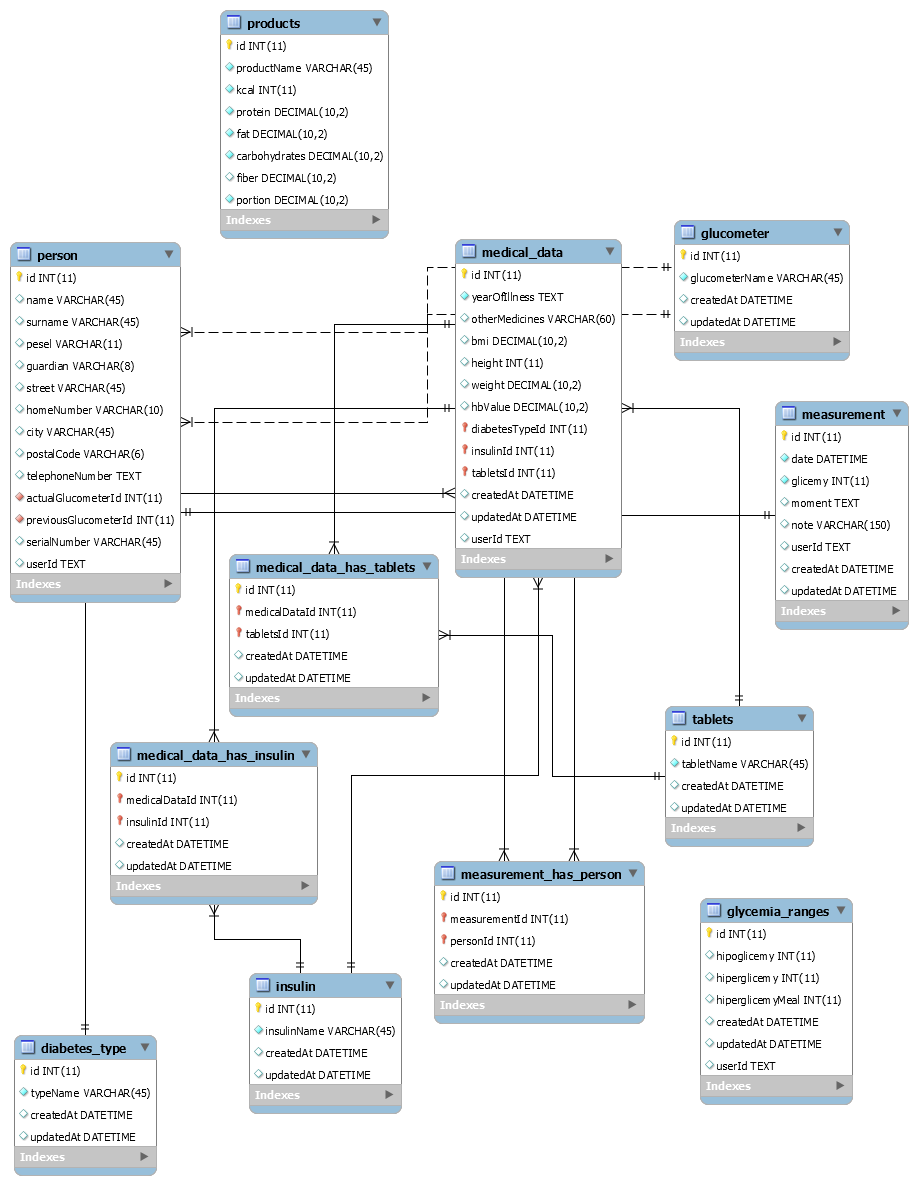
\includegraphics[scale=0.5]{images/dialog_eer.png}
	\caption{Diagram EER bazy danych aplikacji}
	\label{Rys:diagram-eer}
\end{figure}

Zapytania do bazy danych generowane są w sposób automatyczny za pomocą ORM \textit{Sequelize} na podstawie odwzorowanego w kodzie źródłowym modelu bazy danych. Cała baza danych w~ programie została wygenerowana w konwecji \textit{Code First} -- najpierw stworzony był model, a następnie na podstawie tego modelu odpowiadająca mu tabela bazy danych. Poniższy kod przedstawia przykładową implementację modelu tabeli \textit{products}:

\begin{verbatim}
module.exports = function(sequelize, DataTypes) {
	return sequelize.define('products', {
	id: {
	type: DataTypes.INTEGER(11),
	allowNull: false,
	primaryKey: true,
	autoIncrement: true
	},
	productName: {
	type: DataTypes.STRING(45),
	allowNull: false
	},
	kcal: {
	type: DataTypes.INTEGER(11),
	allowNull: false
	},
	protein: {
	type: DataTypes.DECIMAL,
	allowNull: false
	},
	fat: {
	type: DataTypes.DECIMAL,
	allowNull: false
	},
	carbohydrates: {
	type: DataTypes.DECIMAL,
	allowNull: false
	},
	fiber: {
	type: DataTypes.DECIMAL,
	allowNull: true
	},
	portion: {
	type: DataTypes.DECIMAL,
	allowNull: false
	}
	}, {
	tableName: 'products',
	timestamps : false
	});
	};
}
\end{verbatim}

Początkowo eksportowany jest model przy użyciu funkcji ORM \textit{Sequelize}. Zwracana wartość zawiera odwzorowanie tabeli produkt, na podstawie którego generowane są później automatyczne zapytania do bazy danych. Każde pole tabeli opisywane jest w następujący sposób:

\begin{verbatim}
nazwa_pola: {
	type: typ_pola,
	...
	//odpowiednie opcje i ograniczenia
}
\end{verbatim}

Ograniczenia jakie zostały użyte do zdefiniowania klucza głównego to:

	\begin{verbatim}
	allowNull: false;
	primaryKey: true;
	autoIncrement: true;
	\end{verbatim}

Pierwsze z nich określa czy pole tabeli może być wartością pustą (\textit{NULL}). Klucz główny nie może być wartością pustą, dlatego wartość ta jest ustawiona na \textit{false}. Następna wartość określa czy dane pole jest kluczem głównym. W tym przypadku przyjmuje ono wartość \textit{true}. Ostatnim z~ pól jest określenie autoinkrementowania wartości \textit{id}, dlatego również przyjmuje ono wartość \textit{true}. Ostatni znacznik:

	\begin{verbatim}
	timestamps: false
	\end{verbatim}
określa anulowanie możliwości korzystania z automatycznych znaczników czasu tworzonych w momencie edycji \textit{UPDATE} tabeli.
